\chapter{Kerberos} 
\section{Introducci\'on}
Durante 1983 en el M.I.T. ({\it Massachussetts Institute of Technology}) 
comenz\'o el proyecto {\it Athena} con el objetivo de crear un entorno de
trabajo educacional compuesto por estaciones gr\'aficas, redes de alta velocidad
y servidores; el sistema operativo para implementar este entorno era Unix 
4.3BSD, y el sistema de autenticaci\'on utilizado en el proyecto se denomin\'o 
{\it Kerberos} (\cite{kn:mil87}) en honor al perro de tres cabezas que en la 
mitolog\'{\i}a griega vigila la puerta de entrada a Hades, el infierno.\\
\\Hasta que se dise\~n\'o {\it Kerberos}, la autenticaci\'on en redes de 
computadores se realizaba principalmente de dos formas: o bien se aplicaba la
autenticaci\'on por declaraci\'on ({\it Authentication by assertion}), en la que
el usuario es libre de indicar el servicio al que desea acceder (por ejemplo,
mediante el uso de un cliente determinado), o bien se utilizaban contrase\~nas
para cada servicio de red. Evidentemente el primer modelo proporciona un nivel
de seguridad muy bajo, ya que se le otorga demasiado poder al cliente sobre el
servidor; el segundo modelo tampoco es muy bueno: por un lado se obliga al
usuario a ir tecleando cont\'{\i}nuamente su clave, de forma que se pierde 
demasiado tiempo y adem\'as la contrase\~na est\'a viajando cont\'{\i}nuamente
por la red. {\it Kerberos} trata de mejorar estos esquemas intentando por un
lado que un cliente necesite autorizaci\'on para comunicar con un servidor
(y que esa autorizaci\'on provenga de una m\'aquina confiable), y por otro
eliminando la necesidad de demostrar el conocimiento de informaci\'on privada
(la contrase\~na del usuario) divulgando dicha informaci\'on.\\
\\{\it Kerberos} se ha convertido desde entonces en un referente obligatorio a
la hora de hablar de seguridad en redes. Se encuentra disponible para la 
mayor\'{\i}a de sistemas Unix, y viene integrado con OSF/DCE ({\it Distributed 
Computing Environment}). Est\'a especialmente recomendado para sistemas 
operativos distribuidos, en los que la autenticaci\'on es una pieza fundamental 
para su funcionamiento: si conseguimos que un servidor logre conocer la 
identidad de un cliente puede decidir sobre la concesi\'on de un servicio o la 
asignaci\'on de privilegios especiales. Sigue vigente en la actualidad (en su
versi\'on V a la hora de escribir este trabajo), a pesar del tiempo 
transcurrido desde su dise\~no; adem\'as fu\'e el pionero de los sistemas 
de autenticaci\'on para sistemas en red, y muchos otros dise\~nados 
posteriormente, como {\it 
KryptoKnight} (\cite{kn:mol92}, \cite{kn:jan97}\dots), {\sc sesame} 
(\cite{kn:pin93}) o {\it Charon} (\cite{kn:atk93}) se basan en mayor o menor 
medida en {\it Kerberos}.\\
\\El uso de {\it Kerberos} se produce principalmente en el {\it login}, en el 
acceso a otros servidores (por ejemplo, mediante {\tt rlogin}) y en el acceso
a sistemas de ficheros en red como {\sc nfs}. Una vez que un cliente est\'a
autenticado o bien se asume que todos sus mensajes son fiables, o si se desea
mayor seguridad se
puede elegir trabajar con mensajes seguros (autenticados) o privados
(autenticados y cifrados). {\it Kerberos} se puede implementar en un 
servidor que se ejecute en una m\'aquina segura, mediante un conjunto de 
bibliotecas que utilizan tanto los clientes como las aplicaciones; se trata de
un sistema
f\'acilmente escalable y que admite replicaci\'on, por lo que se puede utilizar
incluso en sistemas de alta disponibilidad (aunque como veremos al final del
cap\'{\i}tulo est\'a fuertemente centralizado).
\section{Arquitectura de Kerberos}
Un servidor {\it Kerberos} se denomina KDC ({\it Kerberos Distribution Center}),
y provee de dos servicios fundamentales: el de autenticaci\'on (AS, {\it 
Authentication Service}) y el de {\it tickets} (TGS, {\it Ticket Granting 
Service}). El primero tiene como funci\'on autenticar inicialmente a los 
clientes y proporcionarles un {\it ticket} para comunicarse con el segundo, 
el servidor de {\it tickets}, que proporcionar\'a a los clientes las 
credenciales necesarias para comunicarse con un servidor final que es quien
realmente ofrece un servicio. Adem\'as, el servidor posee una base de datos de
sus clientes (usuarios o programas) con sus respectivas claves privadas, 
conocidas \'unicamente por dicho servidor y por el cliente que al que 
pertenece.\\
\\La arquitectura de {\it Kerberos} est\'a basada en tres objetos de seguridad:
Clave de Sesi\'on, {\it Ticket} y Autenticador.
\begin{itemize}
\item{}
La {\bf clave de sesi\'on} es una clave secreta generada por {\it Kerberos} y
expedida a un cliente para uso con un servidor durante una sesi\'on; no es
obligatorio utilizarla en toda la comunicaci\'on con el servidor, s\'olo si el
servidor lo requiere (porque los datos son confidenciales) o si el servidor es
un servidor de autenticaci\'on. Se suele denominar a esta clave $K_{CS}$,
para la comunicaci\'on entre un cliente C y un servidor S.\\
Las claves de sesi\'on se utilizan para minimizar el uso de las claves secretas
de los diferentes agentes: \'estas \'ultimas son v\'alidas durante mucho
tiempo, por lo que es conveniente para minimizar ataques utilizarlas lo menos 
posible.
\item{}
El {\bf ticket} es un testigo expedido a un cliente del servicio de {\it
tickets} de {\it Kerberos} para solicitar
los servicios de un servidor; garantiza que el cliente ha sido autenticado
recientemente. A un {\it ticket} de un cliente C para acceder a un servicio S
se le denomina
$\{ticket(C,S)\}_{K_{S}}\, =\, \{C, S, t_{1}, t_{2}, K_{CS}\}_{K_{S}}$.
Este {\it ticket} incluye el nombre del cliente C, para evitar su posible uso
por impostores, un periodo de validez $[t_{1},t_{2}]$ y una clave de sesi\'on
$K_{CS}$ asociada para uso de cliente y servidor. {\it Kerberos} siempre
proporciona el {\it ticket} ya cifrado con la clave secreta del servidor al que
se le entrega.
\item{}
El {\bf autenticador} es un testigo construido por el cliente y enviado a un
servidor para probar su identidad y la actualidad de la comunicaci\'on; s\'olo
puede ser utilizado una vez. Un autenticador de un cliente C ante un servidor S
se denota por $\{auth(C)\}_{K_{CS}}\, = \, \{C,t\}_{K_{CS}}$.
Este autenticador contiene, cifrado con la clave de la sesi\'on, el nombre del
cliente y un {\it timestamp}.\\
\end{itemize}
{\it Kerberos} sigue de cerca el protocolo de Needham y Schroeder
(\cite{kn:nee78}) con clave
secreta, utilizando {\it timestamps} como pruebas de frescura con dos
prop\'ositos: evitar reenv\'{\i}os de viejos mensajes capturados en la red o la
reutilizaci\'on de viejos {\it tickets} obtenidos de zonas de memoria del
usuario autorizado, y a la vez poder revocar a los usuarios los derechos al
cabo de un tiempo.
\section{Autenticaci\'on}
El protocolo de autenticaci\'on de {\it Kerberos} es un proceso en el que
diferentes elementos colaboran para conseguir identificar a un cliente que 
solicita un servicio ante un servidor que lo ofrece; este proceso se
realiza en tres grandes etapas que a continuaci\'on se describen. En la tabla 
\ref{kerb-abbr} se muestran las abreviaturas utilizadas, y en la figura 
\ref{kerb} un resumen gr\'afico de este protocolo.
\begin{table}
\begin{center}
\begin{tabular}{|c||c|}
\hline
C & Cliente que solicita un servicio\\
\hline
S & Servidor que ofrece dicho servicio\\
\hline
A & Servidor de autenticaci\'on\\
\hline
T & Servidor de {\it tickets}\\
\hline
K$_{C}$ & Clave secreta del cliente\\
\hline
K$_{S}$ & Clave secreta del servidor\\
\hline
K$_{T}$ & Clave secreta del servidor de {\it tickets}\\
\hline
K$_{CT}$ & Clave de sesi\'on entre el cliente y el servidor de {\it tickets}\\
\hline
K$_{CS}$ & Clave de sesi\'on entre cliente y servidor\\
\hline
\end{tabular}
\caption{Abreviaturas utilizadas.}
\label{kerb-abbr}
\end{center}
\end{table}
\subsection{Login}
Inicialmente el cliente C (en este caso el usuario a trav\'es del programa {\tt
login}) necesita obtener las
credenciales necesarias para acceder a otros servicios. Para ello 
cuando un usuario conecta a un sistema Unix `kerberizado' teclea en primer 
lugar su nombre de usuario, de la misma forma que en un sistema habitual; la
diferencia est\'a en que el programa {\tt login} env\'{\i}a el nombre de
usuario al servidor de autenticaci\'on de {\it Kerberos} para solicitar un {\it
ticket} que le permita comunicarse posteriormente con el servidor de {\it 
tickets}, TGS:
\begin{center}
$C\,\rightarrow\, A:\, C,T,N$
\end{center}
Si el usuario es conocido, el servidor de autenticaci\'on retorna un mensaje 
que contiene una clave para 
la comunicaci\'on con TGS y un {\it timestamp} cifrado con la clave secreta del 
cliente, junto un {\it ticket} para la comunicaci\'on 
con TGS cifrado con la clave secreta de este servidor:
\begin{center}
$A\,\rightarrow\, C:\,\{K_{CT},N\}_{K_{C}}\, ,\, \{ticket(C,T)\}_{K_{T}}$
\end{center}
El programa de {\it login} intentar\'a descifrar $\{{K_{CT},N}\}_{K_{C}}$, con 
la clave que el usuario proporciona, y si \'esta es correcta podr\'a obtener 
$K_{CT}$ y $N$: un cliente s\'olo podr\'a descifrar esta parte del mensaje si 
conoce su 
clave secreta, $K_{C}$ (en este caso el {\it password}). Una vez obtenida
$K_{CT}$, la clave para comunicar al cliente con el servidor de {\it tickets}, 
el programa {\tt passwd} la guarda para una posterior comunicaci\'on
con el TGS y borra la clave del usuario de memoria, ya que el {\it ticket} 
ser\'a suficiente para autenticar al cliente; este modelo consigue que {\bf el
{\it password} nunca viaje por la red}.
\subsection{Obtenci\'on de {\it tickets}}
El cliente ya posee una clave de sesi\'on para comunicarse con el servidor de
{\it tickets} y el {\it ticket} necesario para hacerlo, cifrado con la clave 
secreta de este servidor (el cliente {\bf no} puede descifrar este {\it 
ticket}). Cuando el cliente necesita acceder a un determinado servicio es 
necesario que disponga de un {\it ticket} para hacerlo, por lo que lo solicita 
al TGS envi\'andole un autenticador que el propio cliente genera, el {\it
ticket} de T y el nombre del servicio al que desea acceder, S, y un indicador
de tiempo:
\begin{center}
$C\,\rightarrow\, T:\,\{auth(C)\}_{K_{CT}}\, ,\, \{ticket(C,T)\}_{K_{T}}\, ,\, S\, ,\, N$
\end{center}
Cuando TGS recibe el {\it ticket} comprueba su validez y si todo es correcto
retorna un mensaje que contiene una clave para comunicaci\'on con S y un {\it 
timestamp} cifrado con la clave de sesi\'on del par CT, junto a un {\it ticket} 
para que el cliente C y el servidor S se puedan comunicar cifrado con la 
clave secreta del servidor:
\begin{center}
$T\,\rightarrow\, C:\,\{K_{CS},N\}_{K_{CT}}\, ,\, \{ticket(C,S)\}_{K_{S}}$
\end{center}
C s\'olo podr\'a obtener $K_{CS}$ si conoce la clave secreta, $K_{CT}$.
\subsection{Petici\'on de servicio}
Tras obtener el {\it ticket} para comunicarse con S el cliente ya est\'a
preparado para solicitar el servicio; para ello presenta la credencial
autenticada ante el servidor final, que es quien va a prestar el servicio.
C se comporta de la misma forma que cuando solicit\'o un {\it ticket} a T: 
env\'{\i}a a S el autenticador reci\'en generado, el {\it ticket} y una 
petici\'on que puede ir cifrada si el servidor lo requiere, aunque no es 
necesario:
\begin{center}
$C\,\rightarrow\, S:\,\{auth(C)\}_{K_{CS}}\, ,\, \{ticket(C,T)\}_{K_{S}}\, ,\,
peticion\, ,\,N$
\end{center}
El servidor env\'{\i}a entonces al cliente la prueba de actualidad cifrada con 
la clave secreta de la sesi\'on:
\begin{center}
$S\,\rightarrow\, C:\,\{N\}_{K_{CS}}$
\end{center}
S\'olo S pudo obtener $K_{CS}$ y por tanto enviar este mensaje.
\begin{figure}
\fbox{
%\parbox{6.7in}{
\parbox{\textwidth}{
\begin{center}
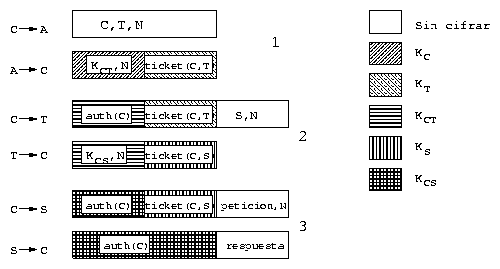
\includegraphics[width=\textwidth]{kerby.png}
\end{center}
}}
\caption{Protocolo de autenticaci\'on {\it Kerberos}.}
\label{kerb}
\end{figure}
\section{Problemas de Kerberos}
A la vista de todo lo comentado en los puntos anteriores puede darnos la
impresi\'on de que {\it Kerberos} es la panacea de los sistemas de 
autenticaci\'on. Sin embargo, y aunque se trate de un sistema robusto, no est\'a
exento de ciertos problemas, tanto de seguridad como de implementaci\'on, que
han hecho que este sistema no est\'e todo lo extendido que deber\'{\i}a.\\
\\Uno de los principales problemas de {\it Kerberos} es que cualquier programa
que lo utilice ha de ser modificado para poder funcionar correctamente, 
siguiendo un proceso denominado `kerberizaci\'on'. Esto implica obviamente que
se ha de disponer del c\'odigo fuente de cada aplicaci\'on que se desee 
kerberizar, y tambi\'en supone una inversi\'on de tiempo considerable para 
algunas aplicaciones m\'as o menos complejas que no todas las organizaciones se
pueden permitir.\\
\\El problema anterior es simplemente de implementaci\'on; no afecta para nada
a la seguridad -- o inseguridad -- del protocolo. Un problema que s\'{\i} est\'a
relacionado con la seguridad de {\it Kerberos} es la gran centralizaci\'on que
presenta el sistema. Para un correcto funcionamiento se ha de disponer en todo
momento del servidor {\it Kerberos}, de forma que si la m\'aquina que lo alberga
falla, la red se convierte en inutilizable; obviamente esto es una 
contradicci\'on con lo que nos dice la teor\'{\i}a de sistemas distribuidos, 
donde se recalca el uso de la distribuci\'on para mantener la disponibilidad del
sistema, intentado que si un equipo falla el resto pueda seguir funcionando, si
no a pleno rendimiento, al menos correctamente. Por si esto no fuera suficiente,
otro ejemplo de la centralizaci\'on de {\it Kerberos} reside en el hecho de que
casi toda la seguridad reside en el servidor que mantiene la base de datos de
claves, de forma que si \'este se ve comprometido, la red entera est\'a 
amenazada.\\
\\Otro potencial problema de seguridad es el uso de {\it timestamps} como 
pruebas de frescura en {\it Kerberos}. Esto obliga a que todas las m\'aquinas
que ejecutan servicios autenticados mantengan sus relojes m\'{\i}nimamente
sincronizados (con desfases m\'aximos de pocos minutos), con todo lo que esto
implica. Adem\'as ese tiempo global ha de ser accesible a todas las estaciones;
aunque en el dise\~no no se asume que todas mantengan la hora exacta, s\'{\i} 
que se les obliga a mantenerse dentro de los m\'argenes si desean solicitar
{\it tickets}, para lo que se necesitan servidores de tiempo con los que los
clientes puedan sincronizar peri\'odicamente sus relojes, por ejemplo cada
vez que arrancan.\\
\\Todos estos problemas, y algunos m\'as (\cite{kn:bel91}) que se han ido 
solucionando en diferentes versiones del sistema, han propiciado que el uso de 
{\it Kerberos} no est\'e muy extendido; en la mayor\'{\i}a de redes es 
suficiente con un protocolo de comunicaci\'on cifrado para mantener una 
m\'{\i}nima seguridad, de forma que el complejo modelo de {\it Kerberos} se ve 
sustituido a ese efecto por programas tan simples y transparentes como {\sc 
ssh}.
